\section{Úvod do funkcionální analýzy}


V této kapitole se budeme zabývat prostory funkcí, v nichž je vhodné hledat slabé řešení.
Teorie těchto abstraktních prostorů je poměrně obsáhlá, pro zájemce o hlubší poznatky odkazujeme na knihu \cite{rektorys1974variacni}.
% pojmy jako norma a limita v abstraktních budeme studovat některé vlastnosti pojmů jako metrika, norma nebo skalární součin.


\subsection{Normované lineární prostory}

Pojmy skalární součin a norma lze zavést na různých množinách, např. na množině matic nebo reálných funkcí.
\begin{df}
Nechť $V$ je vektorový prostor.
\begin{itemize}
\item[(i)] Řekneme, že zobrazení $l:V\to\Real$ je \emph{lineární forma} na $V$, pokud pro každé $u,v\in V$ a~$\alpha,\beta\in\Real$ platí:
\[ l(\alpha u+\beta v) = \alpha l(u) + \beta l(v). \]
\item[(ii)] Zobrazení $a:V\times V\to\Real$ nazveme \emph{bilineární formou}, pokud $a$ je lineární v obou proměnných, tj.
\[ a(u,\alpha v+\beta w) = \alpha a(u,v) + \beta a(u,w), \qquad
 a(\alpha u+\beta v,w) = \alpha a(u,v) + \beta a(v,w) \]
pro každé $u,v,w\in V$ a $\alpha,\beta\in\Real$.
\item[(iii)] Bilineární forma $a$ se nazývá \emph{symetrická}, pokud
\[ \forall u,v\in V:~a(u,v)=a(v,u). \]
\item[(iv)] \emph{Skalární součin} je symetrická bilineární forma $a$, která splňuje
\[ \forall v\in V,~v\neq \0:~a(v,v)>0. \]
\item[(v)] \emph{Norma indukovaná skalárním součinem} $a$ je definována výrazem
\[ \norm{v}_a := \left(a(v,v)\right)^{1/2},~v\in V. \]
\end{itemize}
\end{df}
Pro indukovanou normu platí \emph{Cauchyova-Schwarzova nerovnost}:
\[ \forall v,w\in V: ~|a(v,w)| \le \norm{v}_a\norm{w}_a. \]
Norma obecně nemusí být indukovaná skalárním součinem, musí však splňovat následující vlastnosti.
\begin{df}
Funkce $\norm{\cdot}:V\to\R$ se nazývá \emph{norma} na vektorovém prostoru $V$, pokud pro každé $u,v\in V$ a $\alpha\in\R$ platí:
\begin{itemize}
\item[(i)] $\norm{u}=0 ~\Leftrightarrow~u=\vec 0$,
\item[(ii)] $\norm{\alpha u}=|\alpha|\norm{u}$,
\item[(iii)] $\norm{u+v}\le\norm{u}+\norm{v}$.
\end{itemize}
Je-li na $V$ definována norma, nazývá se $V$ \emph{normovaný lineární prostor}.
\end{df}
Z definice normy vyplývá, že může nabývat jen nezáporných hodnot (dokažte!).


\begin{ex}
Na množině $\R^n$, $n\in\N$, lze zavést normu $\norm{(x_1,\ldots,x_n)}_p:=\left(\sum_{i=1}^n|x_i|^p\right)^{1/p}$, $p\in[1,\infty)$, nebo $\norm{(x_1,\ldots,x_n)}_\infty:=\max_{i=1,\ldots,n}|x_i|$. Norma $\norm{\cdot}_2$ je indukovaná standardním skalárním součinem vektorů.
\end{ex}

V dalším textu bude $\Omega$ oblast (otevřená souvislá množina) v $\R^d$, $d\in\{1,2,3\}$.
Pro zjednodušení některých úvah také budeme předpokládat, že $\Omega$ je omezená.
Hranici $\Omega$ budeme značit symbolem $\partial\Omega$ a uzávěr symbolem $\overline\Omega:=\Omega\cup\partial\Omega$.

\begin{ex}
Na prostoru spojitých funkcí $C(\overline\Omega)$ definujeme skalární součin
\[ (u,v):=\int_\Omega u(x) v(x)~dx \]
a jím indukovanou normu
\[ \norm{u}_2 := \sqrt{(u,u)} = \left(\int_\Omega u^2(x)~dx\right)^{1/2}. \]
Lze také zavést normu
\[ \norm{u}_\infty := \max_{x\in\overline\Omega}|u(x)|. \]
\end{ex}

\begin{ex}
Na prostoru spojitě diferencovatelných funkcí
\[ C^1(\overline\Omega):=\left\{u\in C(\overline\Omega);~\forall i=1,\ldots,d~\frac{\partial u}{\partial x_i}\in C(\overline\Omega)\right\} \]
definujeme skalární součin
\[ ((u,v)) := (u,v) + \sum_{i=1}^d(\frac{\partial u}{\partial x_i},\frac{\partial v}{\partial x_i}), \]
který indukuje normu
\[ \norm{u}_{1,2} := \sqrt{((u,u))} = \left(\int_\Omega u^2 + \sum_{i=1}^d\left|\frac{\partial u}{\partial x_i}\right|^2~dx\right)^{1/2}. \]
Mimo to existuje také norma
\[ \norm{u}_{1,\infty} := \max\left\{\norm{u}_{\infty},\norm{\frac{\partial u}{\partial x_1}}_{\infty},\dots,\norm{\frac{\partial u}{\partial x_d}}_\infty\right\}. \]
\end{ex}

\begin{ex}
Uvažujme funkci
\[ u(x):=\begin{cases}10\sin(1000\pi x) & \mbox{ pro }x\in[0,\frac1{1000}]\\0 & \mbox{ jinak}\end{cases}. \]
Snadno lze spočítat:
\[
\norm{u}_2 = \sqrt{\int_0^{1/1000}100\sin^2(1000\pi x)~dx}
= \sqrt{100\left[\frac{x}2-\frac{\sin(2000\pi x)}{4000\pi}\right]_{x=0}^{1/1000}}
= \frac1{2\sqrt{5}}\doteq 0,224,
\]
\[ \norm{u}_\infty = \max_{x\in[0,1/1000]}|10\sin(1000\pi x)| = 10. \]
\end{ex}

Norma $\norm{\ }_\infty$ se zdá být v jistém smyslu přirozenější, neboť měří maximální odchylku hodnot dvou spojitých funkcí.
Přesto existují důvody, proč je vhodné používat normu $\norm{\ }_2$.
Předně, $\norm{\ }_2$ byla zavedena pomocí skalárního součinu. Skalární součin hraje v některých úlohách důležitou roli.
Lze ukázat, že na množině spojitých funkcí nelze zavést skalární součin s rozumnými vlastnostmi, který by indukoval normu $\norm{\cdot}_\infty$.
Dalším důvodem je, že v mnoha aplikacích nevystačíme se spojitými funkcemi. Není snadné rozšířit normu $\norm{\ }_\infty$ na obecnější třídu funkcí, zatímco rozšíření normy $\norm{\ }_2$ je velmi jednoduché a vede přirozeně k vytvoření tzv. prostoru $L^2$.





% \subsubsection{Hustá množina, separabilní prostor}
% 
% Metrické prostory obecně nemají lineární strukturu jako vektorové prostory.
% Nelze v nich proto definovat bázi.
% Každý metrický prostor ale obsahuje podmnožinu, jejímiž prvky lze aproximovat libovolný prvek.
% \begin{df}
% Řekneme, že množina $M\subset X$ je \emph{hustá} v metrickém prostoru $(X,\varrho)$, pokud $\overline M=X$.
% \end{df}
% Je-li $M$ hustá množina, pak pro každý prvek $x\in X$ existuje posloupnost $\{x_n\}$ prvků $M$ taková, že
% \[ x_n\to x. \]
% \begin{veta}
% Množina všech polynomů je hustá v $L^p(\Omega)$, $p\in[1,\infty)$.
% \end{veta}
% Důsledkem předchozí věty je, že ke každé funkci $f\in L^p(\Omega)$ a pro libovolné $\varepsilon>0$ existuje polynom $f_\varepsilon$, který je vzdálen od $f$ o méně než $\varepsilon$:
% \[ \norm{f-f_\varepsilon}_p < \varepsilon. \]
% Množina všech polynomů je ovšem poměrně velká (obsahuje nespočetně mnoho funkcí).
% \begin{df}
% Řekneme, že metrický prostor je \emph{separabilní}, jestliže v něm existuje hustá množina, která je nanejvýš spočetná.
% \end{df}
% Jestliže je prostor separabilní, pak lze najít posloupnost jeho prvků, které tvoří hustou množinu.
% \begin{veta}
% Prostor $(L^p(\Omega),\varrho_p)$, $p\in[1,\infty)$, a prostoru $(C(\overline\Omega),\varrho_\infty)$ je separabilní.
% \end{veta}
% Příkladem spočetné husté množiny v $L^p(\Omega)$, resp. v $C(\overline\Omega)$, je množina všech polynomů s racionálními koeficienty.







\subsubsection{Konvergence}
% 
\begin{df}
Nechť $V$ je normovaný lineární prostor. Řekneme, že posloupnost $\{u_n\}_{n\in\N}$ prvků z $V$ \emph{konverguje} k $u\in V$ v normě, jestliže
\[ \lim_{n\to\infty} \norm{u_n-u} = 0. \]
Říkáme, že $u$ je limita posloupnosti $\{u_n\}$ a píšeme
\[ u=\lim_{n\to\infty} u_n \mbox{ ve }V, \mbox{ nebo }u_n\to u \mbox{ ve }V. \]
\end{df}
% 
Pro limitu v normovaném lineárním prostoru platí obdobná tvrzení jako pro limitu v $\R^n$ známá ze základních kurzů matematiky.
Např. každá posloupnost má nejvýše jednu limitu.
Pokud posloupnost spojitých funkcí $\{u_n\}$ konverguje k $u$ v normě $\norm{\ }_2$ nebo $\norm{\ }_\infty$, pak prvek $u$ se skoro všude shoduje s bodovou limitou, tj.
\[ (\lim_{n\to\infty} u_n)(x) = \lim_{n\to\infty} (u_n(x)). \]
Pro zjišťování konvergence posloupnosti funkcí je tedy vhodné nejprve zjistit, zda existuje bodová limita.

\begin{ex}
\label{ex:conv_l2_linf}
Uvažujme posloupnost funkcí $\{u_n\}$,
\[ u_n(x) := \begin{cases}10\sin(n\pi x) & \mbox{ pro }x\in[0,\frac1n]\\0 & \mbox{ jinak}\end{cases} \]
v prostoru $C([0,1])$.
Pro ověření, zda má daná posloupnost limitu, nejprve potřebujeme vhodného ``kandidáta''.
Spočteme proto nejprve bodovou limitu.
Zřejmě $\lim u_n(0)=0$.
Je-li $x\in(0,1]$, pak lze najít číslo $n_0\in\N$ takové, že $x>\frac1{n_0}$, takže pro $n\ge n_0$ platí $u_n(x)=0$, a proto musí být $\lim u_n(x) = 0$.
Bodová limita posloupnosti je tedy nulová funkce.
Lze ukázat, že
\[ \norm{u_n-0}_2 = \sqrt{\frac{50}n}, \mbox{ takže }\lim \norm{u_n-0}_2=0, \]
a tedy
\[ \lim u_n = 0 \mbox{ v prostoru }C([0,1]) \mbox{ s normou }\norm{\ }_2. \]
Dále platí
\[ \norm{u_n-0}_\infty = 10, \]
z čehož plyne, že v prostoru $C([0,1])$ s normou $\norm{\ }_\infty$ není nulová funkce limitou posloupnosti $\{u_n\}$ (ve skutečnosti posloupnost není v tomto prostoru konvergentní).
\end{ex}
% 
Uvedený příklad poukazuje na to, že existence limity v metrickém prostoru závisí na tom, jakou uvažujeme metriku.
% Obecně tedy ta samá posloupnost může být v jedné metrice konvergentní a v jiné ne.
\begin{df}
Nechť $\norm{\ }_A$ a $\norm{\ }_B$ jsou normy na prostoru $V$.
Jestliže existují konstanty $\alpha,\beta>0$ takové, že pro každé $u\in V$ platí
\[ \alpha\norm{u}_A \le \norm{u}_B \le \beta\norm{u}_A, \]
pak říkáme, že $\norm{\ }_A$ a $\norm{\ }_B$ jsou na $V$ \emph{ekvivalentní}.
\end{df}
% 
Jsou-li normy $\norm{\ }_A$ a $\norm{\ }_B$ ekvivalentní, pak platí
\[ u_n\to u \mbox{ ve }(V,\norm{\ }_A) \quad \Leftrightarrow \quad u_n\to u \mbox{ ve }(V,\norm{\ }_B). \]
% Ekvivalentní normy také generují stejné otevřené a uzavřené množiny.
Příklad \ref{ex:conv_l2_linf} ukazuje, že normy $\norm{\ }_2$ a $\norm{\ }_\infty$ nejsou na prostoru $C(\overline\Omega)$ ekvivalentní.


\subsubsection{Úplnost}
% 
Skutečnost, že daná posloupnost v metrickém prostoru je konvergentní, závisí nejen na zvolené metrice, ale také na prostoru samotném.
Existují například posloupnosti racionálních čísel, které mají za limitu iracionální číslo, tzn., že jsou konvergentní v prostoru $\R$, ale nejsou konvergentní v $\Q$.
Množina $\Q$ tedy v jistém smyslu není úplná.

Pojem úplnost souvisí s cauchyovskými posloupnostmi.
% 
\begin{df}
Posloupnost $\{u_n\}$ v normovaném lineárním prostoru $V$ se nazývá \mbox{cauchyovská}, jestliže
\[ \forall\varepsilon>0~\exists N\in\N~\forall m,n\in\N:~m,n>N\Rightarrow \norm{u_m-u_n}<\varepsilon. \]
\end{df}
% 
% Vzdálenost prvků cauchyovské posloupnosti tedy může být libovolně malá, jsou-li indexy těchto prvků dostatečně velké.
Cauchyovská posloupnost obecně nemusí mít limitu. Avšak každá konvergentní posloupnost je nutně cauchyovská.
% 
\begin{df}
Normovaný lineární prostor $V$ se nazývá \emph{úplný} (nebo také \emph{Banachův prostor}), jestliže každá cauchyovská posloupnost má v tomto prostoru limitu.
Úplný prostor se skalárním součinem se nazývá \emph{Hilbertův prostor}.
\end{df}
% 
\begin{ex}
Prostory $\R^n$, $n\in\N$, s normami $\norm{\ }_p$, $p\in[1,\infty]$ jsou úplné (díky Bolzanově-Cauchyově podmínce).
Prostor $\Q$ není úplný (např. posloupnost $\{(1+\frac1n)^n\}$ je v něm cauchyovská, ale její limita $e\notin\Q$).
\end{ex}

\begin{ex}
Uvažujme posloupnost $\{u_n\}$ na prostoru $C([-1,1])$ s normou $\norm{\ }_2$, danou vztahem
\[ u_n(x) := \sqrt[2n+1]{x}. \]
Bodová limita posloupnosti je $\sgn x$, což je nespojitá funkce, a proto posloupnost není v daném prostoru konvergentní.
Platí ale
\[ \norm{u_n-\sgn}_2 = \sqrt{\frac2{(n+1)(2n+3)}}, \quad\mbox{ a tedy } \quad \norm{u_n-\sgn}_2\to 0, \]
což znamená, že $\{u_n\}$ je cauchyovská posloupnost.
Prostor $C([-1,1])$ s normou $\norm{\ }_2$ proto není úplný.
Zůstává otázka, zda existuje nějaký větší prostor s normou $\norm{\ }_2$, ve kterém by byla posloupnost $\{u_n\}$ konvergentní.
\end{ex}

\begin{veta}
Prostor $C(\overline\Omega)$ s normou $\norm{\ }_\infty$ je úplný, s normou $\norm{\ }_2$ není úplný.
\end{veta}



\subsubsection{Množiny v normovaném lineárním prostoru}
% 
Podobně jako u euklidovské vzdálenosti v $\R^n$, lze definovat pojmy jako koule, okolí nebo otevřená množina pomocí normy.
\begin{df}
Nechť $X$ je normovaný lineární prostor s normou $\norm{\ }$.
\begin{itemize}
\item \emph{Koule} se středem $x\in X$ a poloměrem $r>0$ je množina
\[ B_r(x) := \{y\in X;~\norm{x-y}<r\}. \]
\item Množina $M$ se nazývá \emph{otevřená}, pokud pro každý bod $x\in M$ existuje koule se středem $x$, která leží v $M$.
\item Množina se nazývá \emph{uzavřená}, pokud její doplněk v $X$ je otevřený.
\end{itemize}
\end{df}

\begin{ex}
Koule v prostoru $\R^2$ se středem v počátku souřadné soustavy má tvar
\begin{itemize}
\item[a)] čtverce, jehož vrcholy leží na souřadných osách a těžiště v počátku, uvažujeme-li normu $\norm{\ }_1$;
\item[b)] kruhu se středem v počátku, uvažujeme-li euklidovskou normu $\norm{\ }_2$;
\item[c)] čtverce, jehož strany jsou rovnoběžné se souřadnými osami a těžiště leží v počátku, uvažujeme-li maximovou normu $\norm{\ }_\infty$.
\end{itemize}
\end{ex}

\begin{df}
Nechť $X$ je normovaný lineární prostor, $x\in X$ a $M\subset M$.
\begin{itemize}
\item Bod $x$ je \emph{vnitřním bodem množiny} $M$, pokud existuje poloměr $r>0$ takový, že $B_r(x)\subset M$.
Množinu všech vnitřních bodů $M$ budeme značit $\Int M$.
\item Bod $x$ je \emph{hraničním bodem množiny} $M$, pokud každá koule se středem v $x$ obsahuje alespoň jeden bod z $M$ a alespoň jeden bod z $X\setminus M$.
Množina všech hraničních bodů $M$ se nazývá \emph{hranice} $M$ a značí se $\partial M$.
\item Uzávěr množiny $M$ je množina $\overline M:=M\cup\partial M$.
\end{itemize}
\end{df}

Mezi právě definovanými množinami platí mnoho vztahů. Např.:
\[ \Int M\subset M \subset \overline M, \quad \Int M\cap \partial M = \emptyset, \]


% \subsubsection{Maticové normy}
% 
% Speciálně zde zmíníme ještě normy na prostoru matic.
% 
% \begin{df}
% Nechť $\norm{\cdot}_X$ značí normu na $\R^n$ a $\norm{\cdot}_Y$ normu na $\R^m$.
% Generovaná norma na prostoru matic $\R^{m\times n}$  je definována vztahem
% \[ \norm{\A}_{XY} := \max_{\xx\in\R^n\setminus\{\vec 0\}}\frac{\norm{\A\xx}_Y}{\norm{\xx}_X} = \max_{\xx\in\R^n,\norm{\xx}_X=1}\norm{\A\xx}_Y. \]
% \end{df}
% Generované normy mají následující vlastnosti:
% \[ \norm{\A\B}_{XY} \le \norm{\A}_{XY}\norm{\B}_{XY},\quad \rho(\A)\le\norm{\A}_{XY},\quad \norm{\mat I}_{XY}=1. \]
% \begin{ex}
% Příklady generovaných maticových norem:
% \begin{itemize}
% \item $\norm{\A}_1:=\max_{\norm{\xx}_1=1}\norm{\A\xx}_1 = \max_{j=1,\ldots,n}\sum_{i=1}^m|a_{ij}|$;
% \item $\norm{\A}_2:=\max_{\norm{\xx}_2=1}\norm{\A\xx}_2 = \sqrt{\rho(\A^\top\A)}$;
% \item $\norm{\A}_\infty:=\max_{\norm{\xx}_\infty=1}\norm{\A\xx}_\infty = \max_{i=1,\ldots,m}\sum_{j=1}^n|a_{ij}|$.
% \end{itemize}
% \end{ex}
% Kromě generovaných norem existuje řada dalších maticových norem.
% Často používaná je tzv. Frobeniova norma
% \[ \norm{\A}_F:=\sqrt{\sum_{i=1}^m\sum_{j=1}^n|a_{ij}|^2}. \]
% Dá se ukázat, že Frobeniova norma není generovaná, přesto však je multiplikativní:
% \[ \norm{\A\B}_F \le \norm{\A}_F\norm{\B}_F. \]
% 





\subsection{Prostory integrovatelných funkcí}

V následující části zavedeme prostor funkcí, který obsahuje spojité funkce a zároveň je úplný vzhledem k normě $\norm{\ }_2$, generované skalárním součinem $(\ ,\ )$.

\begin{df}
\label{df:Lp}
Prostorem $L^2(\Omega)$ rozumíme množinu funkcí
\[ L^2(\Omega):=\left\{u:\Omega\to\R;~\left|\int_\Omega u(x)~dx\right|<\infty,~\norm{u}_2<\infty \right\}. \]
Spolu s normou $\norm{\ }_2$ tvoří $L^2(\Omega)$ normovaný lineární prostor.
% Norma v prostoru $L^p(\Omega)$ je definována výrazem
% \[ \norm{u}_{p,\Omega}:=\left(\int_\Omega|u(x)|^p~dx\right)^{1/p}. \]
\end{df}

% Pokud je zřejmé, na jaké oblasti uvažujeme normu, pak budeme zkráceně psát $\norm{u}_p$.
Z definice plyne, že každá spojitá funkce v $\overline\Omega$ patří do prostorů $L^2(\Omega)$.
Do těchto prostorů ovšem patří i mnoho dalších funkcí, které mohou být nespojité nebo neomezené.

Poznamenejme, že pro správnost některých tvrzení je třeba uvažovat integrály v Definici \ref{df:Lp} v tzv. Lebesgueově smyslu.
Požadavek na integrovatelnost funkce $u$ je splněn pro většinu "kulturních" funkcí (např. pro spojité funkce).
Existují však tzv. neměřitelné funkce, jejichž druhá mocnina je integrovatelná, zatímco funkce samotná ne.


\begin{ex}
Uvažujme funkce
\[ u(x) := \frac1{\sqrt{x}} \quad\mbox{ a }\quad v(x) := \frac1{\sqrt[3]{x}} \]
na intervalu $\Omega:=(0,1)$.
Platí:
% \[ \norm{u}_1 = \int_0^1 \frac1{\sqrt{x}}~dx = \left[2\sqrt{x}\right]_{x=0}^1 = 2, \]
% a tedy $u\in L^1(0,1)$. Na druhou stranu
\[ \norm{u}_2 = \sqrt{\int_0^1 \frac1x~dx} = +\infty, \]
\[ \norm{v}_2^2 = \int_0^1 |v(x)|^2~dx = \int_0^1 \frac1{\sqrt[3]{x^2}}~dx = 3. \]
Proto $u\notin L^2(0,1)$ a $v\in L^2(0,1)$.
% Pokud je oblast $\Omega$ omezená, pak vždy $L^2(\Omega)\subset L^1(\Omega)$, resp. obecněji pro $1\le p\le q<\infty$ platí $L^q(\Omega)\subset L^p(\Omega)$.
\end{ex}

\begin{ex}
Funkce
\[ \sgn x:=\begin{cases}-1 & \mbox{ pro }x<0\\0 & \mbox{ pro }x=0\\1 & \mbox{ pro }x>0\end{cases} \]
je prvkem prostoru $L^2(-1,1)$, neboť
\[ \int_{-1}^1 |\sgn x|^2~dx = \int_{-1}^0 |\sgn x|^2 ~dx + \int_0^1 |\sgn x|^2~dx = \int_{-1}^0 1~dx + \int_0^1 1~dx = 2, \]
a tedy $\norm{\sgn x}_2 = \sqrt{2}$.
Podobně funkce
\[ u(x) := \begin{cases}0 & \mbox{ pro }x\neq 0\\10 & \mbox{ pro }x=0\end{cases} \]
patří do $L^2(-1,1)$ a její norma je $\norm{u}_2=0$.
Vidíme, že norma nezávisí na hodnotě funkce v bodě $x=0$. Dokonce není nutné, aby byla funkce v bodě 0 definována.
\end{ex}

% Do prostoru $L^2(\Omega)$ tedy patří i některé nespojité a neomezené funkce.
Funkce, která je rovna nule všude až na hodnotu v jednom bodě, má nulovou normu a je v jistém smyslu ekvivalentní s nulovou funkcí.
Obecněji postačí, když je funkce nulová všude v $\Omega$ mimo \emph{množinu míry nula}.
Mezi množiny s nulovou mírou patří např. všechny konečné a spočetné množiny.

\begin{df}
Nechť funkce $u,v\in L^2(\Omega)$ jsou si v oblasti $\Omega$ \emph{rovny skoro všude}, tj. všude mimo množinu míry nula (kde se buď jejich hodnoty liší nebo některá z funkcí není definována).
Pak řekneme, že $u$ a $v$ jsou v prostoru $L^2(\Omega)$ \emph{ekvivalentní}.
Píšeme $u=v$ v $L^2(\Omega)$.
\end{df}
Funkce $u$ a $v$ jsou tedy v tomto prostoru pokládány za sobě rovné.
Dvě funkce $u,v$ ekvivalentní v prostoru $L^2(\Omega)$ jsou charakterizovány vlastností
\[ \int_\Omega|u(x)-v(x)|^2~dx = 0. \]

% \begin{veta}[H\"olderova nerovnost]
% Nechť $p,q\in(1,\infty)$ splňují vztah
% \[ \frac1p + \frac1q = 1. \]
% Pak pro každé dvě funkce $u\in L^p(\Omega)$ a $v\in L^q(\Omega)$ platí:
% \[ \left|\int_\Omega u(x)v(x)~dx\right| \le \left(\int_\Omega|u(x)|^p~dx\right)^{1/p} \left(\int_\Omega|v(x)|^q~dx\right)^{1/q}. \]
% \end{veta}

\begin{veta}
Prostor $L^2(\Omega)$ s normou $\norm{\ }_2$ je Banachův prostor.
\end{veta}

Tak jako $L^2(\Omega)$ je nejmenší úplný prostor s normou $\norm{\ }_2$ obsahující $C(\overline\Omega)$, lze zavést také prostor
\[ L^\infty(\Omega):=\left\{u:\Omega\to\R;~\left|\int_\Omega u(x)~dx\right|<\infty, ~\exists C>0:~|u(x)|\le C \mbox{ skoro všude v }\Omega\right\}. \]
Norma na tomto prostoru je
\[ \norm{u}_\infty := \inf\left\{C>0;~|u(x)|\le C \mbox{ skoro všude v }\Omega\right\}. \]
Pro spojité funkce tato definice splývá s původní definicí $\norm{\ }_\infty$.
Také $L^\infty(\Omega)$ je Banachův prostor.
\begin{ex}
Poněkud specifickým případem je tzv. Dirichletova funkce
\[ D(x) = \begin{cases}1;&x\in\Q,\\0;&x\notin\Q.\end{cases} \]
Protože množina $\Q$ racionálních čísel je spočetná, $D$ je skoro všude v $\R$ nulová. Proto
\[ \norm{D}_\infty = 0,\quad \int_{-\infty}^\infty D(x)~dx=0. \]
\end{ex}

Na omezené oblasti $\Omega$ platí následující vztah mezi limitami.
\begin{veta}
Nechť $\Omega$ je omezená oblast v $\R^d$, $d\in\{1,2,3\}$, a $\{u_n\}$ je posloupnost funkcí definovaných v $\Omega$.
Pak platí:
\begin{itemize}
\item[(i)] Jestliže $u_n\to u$ v $L^\infty(\Omega)$, pak $u_n\to u$ také v $L^2(\Omega)$.
\item[(ii)] Jestliže $u_n\to u$ v $L^2(\Omega)$, pak $u_n(x)\to u(x)$ pro skoro všechna $x\in\Omega$.
\end{itemize}
\end{veta}






\subsection{Prostory s integrovatelnými derivacemi}

Pro funkce z prostoru $L^2(\Omega)$ lze zavést pojem derivace.
Uvažujme nejprve funkci $u\in C^1([0,1])$.
Díky pravidlu per partes pak platí pro každé $v\in C^1([0,1])$, $v(0)=v(1)=0$:
\begin{equation}
\label{eq:weak_der_1d}
\int_0^1 u'(x)v(x)~dx = [u(x)v(x)]_{x=0}^1 - \int_0^1u(x)v'(x)~dx = - \int_0^1u(x)v'(x)~dx.
\end{equation}
Jestliže tedy pro nějakou funkci $g$ platí:
\[ \forall v\in C^1([0,1]),~v(0)=v(1)=0:~\int_0^1g(x)v(x)~dx=-\int_0^1 u(x)v'(x)~dx, \]
pak z \eqref{eq:weak_der_1d} víme, že $g=u'$.
Tento poznatek je východiskem pro zavedení tzv. \emph{zobecněné derivace}, která je vhodná i pro funkce $u$, které nemají derivace v klasickém smyslu.
\begin{df}
Nechť $u\in L^2(\Omega)$. Funkce $g\in L^2(\Omega)$ se nazývá \emph{zobecněná parciální derivace} funkce $u$ podle $i$-té proměnné, pokud pro každé $v\in C^1(\overline\Omega)$, $v_{|\partial\Omega}=0$, platí:
\[ \int_\Omega gv = -\int_{\Omega} u\frac{\partial v}{\partial x_i}. \]
Píšeme $g=\frac{\partial u}{\partial x_i}$ v $L^2(\Omega)$.
\end{df}
\begin{ex}
Spočtěme zobecněnou derivaci funkce $u(x):=|x|$ na intervalu $(-1,1)$.
Pro $v\in C^1([-1,1])$, $v(-1)=v(1)=0$ platí:
\begin{multline*}
-\int_{-1}^1|x|v'(x)~dx = -\int_{-1}^0(-x)v'(x)~dx - \int_0^1xv'(x)~dx\\
= [xv(x)]_{x=-1}^0 - \int_{-1}^0v(x)~dx - [xv(x)]_{x=0}^1 + \int_0^1v(x)~dx
= \int_{-1}^1\sgn x v(x)~dx.
\end{multline*}
Je tedy $u'(x)=\sgn x$ v $L^2(-1,1)$.
\end{ex}
\begin{ex}
Uvažujme funkci $u(x) = \sgn x$. Pro $v\in C^1([-1,1])$, $v(-1)=v(1)=0$ platí:
\begin{multline*}
 -\int_{-1}^1u(x)v'(x)~dx = -\int_{-1}^0 (-v'(x))~dx - \int_0^1 v'(x)~dx\\
 = [v(x)]_{x=-1}^0 - [v(x)]_{x=0}^1 = 2v(0) = 2\int_{-1}^1\delta_0(x)v(x)~dx,
\end{multline*}
kde $\delta_0$ se nazývá Diracova $\delta$-funkce (ve skutečnosti to není funkce, ale tzv. \emph{distribuce}). V jistém smyslu tedy platí $(\sgn x)'=2\delta_0(x)$, nicméně $\delta_0\notin L^2(\Omega)$.
\end{ex}
Ne každá funkce z $L^2(\Omega)$ má zobecněnou derivaci v $L^2(\Omega)$.

Pro vektorové funkce $\vc u,\vc v:\Omega\to\R^d$ definujeme
\[ \norm{\vc u}_2 := \left(\sum_{i=1}^d\norm{u_i}_2^2\right)^{1/2},\quad (\vc u,\vc v):=\sum_{i=1}^d(u_i,v_i). \]
Prostor $L^2$ pro vektorové funkce budeme značit $L^2(\Omega;\R^d)$.
\begin{df}
Prostor $H^1(\Omega)$ je množina
\[ H^1(\Omega):=\left\{u\in L^2(\Omega);~\nabla u\in L^2(\Omega;\R^d)\right\}. \]
Na tomto prostoru je definována norma
\[ \norm{u}_{1,2} := \left(\norm{u}_2^2 + \norm{\nabla u}_2^2\right)^{1/2} \]
a skalární součin
\[ ((u,v)):=(u,v) + (\nabla u,\nabla v). \]
\end{df}
\begin{veta}
$H^1(\Omega)$ je Banachův prostor.
\end{veta}

% priklady nespojitych funkci v H1 (2d, 3d)
\begin{ex}
Na oblasti $\Omega=B_1(0)\setminus\{(x,0);~x\in(-1,0)\}$ uvažujme funkci
\[ u(x,y)=\sqrt{r}\sin\frac\theta2,~r=\sqrt{x^2+y^2},~\theta=\arctg\frac xy. \]
Ukážeme, že $u\in H^1(\Omega)$:
\[ \int_\Omega u^2 = \int_{-\pi/2}^{3/2\pi}\int_0^1r^2\sin^2\left(\frac\theta2\right) r~dr~d\theta=\frac\pi4, \]
\[ \nabla u(x,y)=\frac12r^{-3/2}\begin{pmatrix}x\sin\frac\theta2+y\cos\frac\theta2\\y\sin\frac\theta2-x\cos\frac\theta2\end{pmatrix}, \]
\[ \int_\Omega |\nabla u|^2 = \frac14\int_{-\pi/2}^{3/2\pi}\int_0^1 dr~d\theta = \frac\pi2. \]
Přitom podél úsečky $\{(x,0);~x\in(-1,0) \}$ je $u$ nespojitá (obr. \ref{fig:disc_h1}).
\begin{figure}
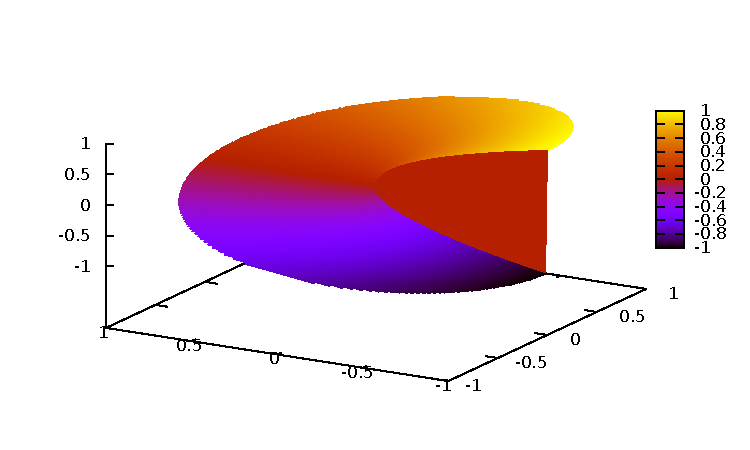
\includegraphics[width=12cm]{discontinuous_h1}
\caption{Nespojitá funkce z prostoru $H^1(\Omega)$.}
\label{fig:disc_h1}
\end{figure}
Pro tuto funkci $u$ nelze jednoznačně definovat hodnoty na hranici $\partial\Omega$.
\end{ex}

Aby bylo možné pro funkce z $H^1(\Omega)$ definovat jejich \emph{stopu}, tj. hodnotu na hranici, omezíme se v dalším na oblasti s \emph{Lipschitzovskou hranicí}.
Řekneme, že oblast $\Omega$ má Lipschitzovskou hranici, jestliže ji lze lokálně popsat jako spojitou funkci s omezenými derivacemi.
% Na prostoru $H^1(\Omega)$ lze definovat hodnoty na hranici prostřednictvím operátoru stop.
Pro funkci $u\in C(\overline\Omega)$ definujeme zobrazení $\tr:u\mapsto u_{|\partial\Omega}$, kde $u_{|\partial\Omega}$ je tzv. stopa funkce $u$ (hodnota na hranici).
Na hranici oblasti $\Omega$, resp. na její části, lze zavést prostor $L^2(\partial\Omega)$ s obdobnými vlastnostmi jako $L^2(\Omega)$.
Normu a skalární součin na hranici budeme značit symbolem $\norm{\ }_{2,\partial\Omega}$, resp. $(\ ,\ )_{\partial\Omega}$.


\begin{veta}[o stopách]\label{th:trace}
Nechť $\Omega$ má Lipschitzovskou hranici. Pak existuje lineární zobrazení $\tr:H^1(\Omega)\to L^2(\partial\Omega)$ s následujícími vlastnostmi:
\[ \forall v\in C(\overline\Omega):~ \tr v = v_{|\partial\Omega}, \]
\[ \forall v\in H^1(\Omega):~\norm{\tr v}_{2,\partial\Omega} \le C\norm{v}_{1,2}, \]
kde konstanta $C>0$ závisí pouze na $\Omega$.
\end{veta}

Poznamenejme, že ne každá funkce z $L^2(\partial\Omega)$ je stopou funkce z $H^1(\Omega)$.
Nyní můžeme zavést prostory funkcí s nulovou stopou:
\begin{df}
Je-li $\Gamma$ relativně otevřená část hranice $\partial\Omega$, pak definujeme
\[ H^1_\Gamma(\Omega) := \{ u\in H^1(\Omega);~\tr u_{|\Gamma}=0 \}. \]
Speciálně pro $\Gamma=\partial\Omega$ značíme tento prostor jako $H^1_0(\Omega)$, tj.
\[ H^1_0(\Omega) := \{ u\in H^1(\Omega);~\tr u=0 \mbox{ na }\partial\Omega\}. \]
\end{df}

% prostory Hk?

\begin{veta}[Friedrichsova nerovnost]\label{th:friedrichs}
Nechť $\Omega$ má Lipschitzovskou hranici a $\Gamma$ je relativně otevřená část $\partial\Omega$.
Pak existuje konstanta $C=C(\Omega,\Gamma)>0$ taková, že pro každé $u\in H^1(\Omega)$ platí nerovnost
\begin{equation} \label{eq:friedrichs_H1gamma}
\norm{u}_{1,2} \le C(\norm{\nabla u}_2 + \norm{u}_{2,\Gamma}).
\end{equation}
Speciálně pro $u\in H^1_0(\Omega)$ platí:
\begin{equation} \label{eq:friedrichs_H10}
\norm{u}_{1,2} \le C\norm{\nabla u}_2.
\end{equation}
\end{veta}

% Greenova veta pro H1






\section{Abstraktní teorie slabých řešení}

V této kapitole se budeme zabývat otázkou, jak správně zavést slabou formulaci tak, aby úloha byla jednoznačně řešitelná.

\subsection{Abstraktní variační úloha}

Nechť $V$ je Hilbertův prostor se skalárním součinem $(\ ,\ )$ a normou $\norm{\ }$, $a$ a $l$ je bilineární, resp. lineární forma na $V$.
Úlohu
\begin{equation}
\label{eq:variational_problem}
\text{Najdi }u\in V \text{ takové, že }\forall v\in V:~a(u,v)=l(v),
\end{equation}
budeme nazývat \emph{abstraktní variační úloha}.

% Lineární forma $l$ je omezená na $V$, pokud existuje konstanta $C>0$ taková, že 
% \[ \forall v\in V:~l(v)\le C\norm{v}. \]
% Bilineární forma $a$ je omezená na $V$, pokud existuje konstanta $C>0$ taková, že 
% \[ \forall u,v\in V:~a(u,v)\le C\norm{u}\norm{v}. \]
% Bilineární forma $a$ je eliptická na $V$, pokud existuje konstanta $\alpha>0$ taková, že
% \[ \forall v\in V:~a(v,v)\ge \alpha\norm{v}^2. \]

\begin{veta}[Lax-Milgram]\label{th:lax-milgram}
Nechť $V$ je Hilbertův prostor, $a$ je bilineární forma na $V$, pro niž existují konstanty $\alpha,\beta>0$ takové, že
\begin{itemize}
\item[(i)] $a$ je omezená, tj.
\[ \forall v,w\in V:~a(v,w)\le \beta\norm{v}\norm{w}, \]
\item[(ii)] $a$ je eliptická na $V$, tj.
\[ \forall v\in V:~\alpha\norm{v}^2\le a(v,v), \]
\end{itemize}
a nechť $l$ je omezená lineární forma na $V$, tj.
\begin{itemize}
\item[(iii)] existuje konstanta $\gamma>0$ taková, že 
\[ \forall v\in V:~l(v)\le \gamma\norm{v}. \]
\end{itemize}
Pak existuje právě jedno řešení $u\in V$ variační úlohy \eqref{eq:variational_problem}.
Navíc platí odhad:
\[ \norm{u} \le \frac\gamma\alpha. \]
\end{veta}


\subsection{Aplikace na eliptické rovnice}


\subsubsection{Nehomogenní Dirichletova podmínka}

Je dána oblast $\Omega\subset\R^d$ a skalární funkce $f$ na $\Omega$ a $u_d$ na $\partial\Omega$.
Hledáme funkci $u:\overline\Omega\to\R$, která splňuje:
\[ 
\begin{aligned}
    -\Delta u &= f &&\text{v }\Omega,\\
    u&=u_d && \text{na }\partial\Omega.
\end{aligned} 
\]
Protože je předepsána Dirichletova podmínka na $\partial\Omega$, prostor, ve kterém budeme hledat slabé řešení, je $V:=H^1_0(\Omega)$.
Jelikož ale hodnota $u$ na hranici je dána funkcí $u_d$, pak obecně $u\notin H^1_0(\Omega)$.
Předpokládejme proto, že $u_d$ lze rozšířit na celou oblast $\Omega$ tak, aby $u_d\in H^1(\Omega)$.
Pak $u-u_d\in H^1_0(\Omega)$.
Řešení budeme hledat ve tvaru $u=z+u_d\in H^1(\Omega)$, kde $z\in H^1_0(\Omega)$, a
\[ 
    \forall v\in H^1_0(\Omega):\ a(z,v)=l(v), 
\]
kde
\begin{equation}\label{eq:def_a_nonhom_dir}
    a(z,v) := (\grad z, \grad v)_{L^2(\Omega)},
\end{equation}
\begin{equation}\label{eq:def_l_nonhom_dir}
    l(v) := (f,v)_{L^2(\Omega)} - (\nabla u_d,\nabla v)_{L^2(\Omega)}.
\end{equation}
% Ukážeme, že formy $a$ a $l$ mají konečnou hodnotu pro každé $u,\varphi\in H^1(\Omega)$.
\begin{veta}
    Pro bilineární formu $a$ definovanou v \eqref{eq:def_a_nonhom_dir} platí:
    \[ \forall v,w\in H^1(\Omega):~a(v,w) \le \norm{v}_{1,2}\norm{w}_{1,2}. \]
    Je-li navíc $f\in L^2(\Omega)$, pak existuje $\gamma:=\norm{f}_2+\norm{\nabla u_d}_2$ takové, že
    \[ \forall v\in H^1(\Omega):~l(v) \le \gamma\norm{v}_{1,2}, \]
    kde lineární forma $l$ je definována v \eqref{eq:def_l_nonhom_dir}.
\end{veta}
\begin{proof}
    Omezenost $a$ plyne přímo z Cauchyovy-Schwarzovy nerovnosti a faktu, že $\norm{\nabla v}_2\le\norm{v}_{1,2}$.
    Dále
    \[ l(v)\le \norm{f}_2\norm{v}_2 + \norm{\nabla u_d}_2\norm{\nabla v}_2
    \le (\norm{f}_2+\norm{\nabla u_d}_2)\norm{v}_{1,2}. \]
\end{proof}


\begin{veta}
    Bilineární forma $a$ je eliptická na $H^1_0(\Omega)$ s konstantou $\alpha=1/C^2$, 
    kde $C=C(\Omega,\partial\Omega)$ je konstanta z Friedrichsovy nerovnosti \eqref{eq:friedrichs_H10}.
\end{veta}
\begin{proof}
    Je-li $v\in H^1_0(\Omega)$, pak
    \[ 
        a(v,v) = (\nabla v,\nabla v)_{L^2(\Omega)} 
               = \norm{\nabla v}_2^2 \ge \frac1{C^2}\norm{v}_{1,2}^2. 
    \]
\end{proof}






\subsubsection{Anizotropní difúze}
Uvažujme úlohu vedení tepla ve čtvercové desce, která je z jedné strany zahřívána infračervenými lampami 
tepelným tokem $f$ a z druhé strany předehřívána ocelovou matricí s tepelnou vodivostí $\sigma$, která je dále 
vyhřívána soustavou kanálků s vodou o teplotě $u_f$. Na dvou stranách čtverce je tepelná izolace, na druhých dvou stranách je 
kostantní teplota $u=0$ (toto je nereálné, ale je to jen příklad). Deska je kompozitní materiál složený z polymerové pryskyřice 
(vodivost 1W/mK) a uhlíkových vláken (vodivost 1000W/mK) s preferovaným směrem, tepelná vodivost desky je proto anisotropní.

Formulujme nyní úlohu abstraktněji.

Mějme oblast $\Omega\subset\R^d$ (například čtverec $d=2$) s hranicí 
$\partial\Omega=\overline\Gamma_d\cup\overline\Gamma_n$, tedy s Dirichletovskou a Neumannovskou částí hranice.
Na této oblasti hledáme teplotu $u:\overline\Omega\to\R$, která je řešením stacionární rovnice vední tepla:
\begin{align}
    -\div(\tn K\grad u) &= f + \sigma(u_f - u) &&\text{v }\Omega,\\
    u&=0 && \text{na }\Gamma_d,\\
    -\tn K \grad u \cdot \vc n &= q &&\text{na }\Gamma_n.
\end{align} 
Zde $\tn K:\Omega\to\R^{d\times d}$ je maticová funkce pro tenzor tepelné vodivosti
a $f$, $\sigma$, $u_f$ jsou skalární funkce na $\Omega$  a $q$ skalární funkce na $\Gamma_n$.

Aby byla splněna Dirichletova podmínka na $\Gamma_d$ a formy $a$, $l$ měly konečnou hodnotu, 
budeme hledat slabé řešení v prostoru 
\[
    V:=H^1_{\Gamma_d}(\Omega) = \{ \phi \in H^1(\Omega),\ \phi = 0\text{ na }\Gamma_d\} 
\]
Nyní převedeme úlohu vedení tepla na abstraktní variační úlohu:
\[ 
    \mbox{Najdi }u\in H^1_{\Gamma_d}(\Omega):~\forall v\in H^1_{\Gamma_d}(\Omega):~a(u,v)=l(v), 
\]
kde formy $a(\cdot, \cdot)$ a $l(\cdot)$ mají tvar:
\begin{equation}\label{eq:def_a_diffusion}
    a(u,v) := (\tn K\grad u, \grad v)_{L^2(\Omega)} + (\sigma u, v)_{L^2(\Omega)},
\end{equation}
\begin{equation}\label{eq:def_l_diffusion}
    l(v) := (f + \sigma u_f,v)_{L^2(\Omega)} - ( q, v)_{L^2(\Gamma_n)}.
\end{equation}
Pro použití Lax-Milgramova lemmatu potřebujeme ověřit omezenost forem $a$ a $l$. To ovšem platí 
za nějakých předpokladů na další parametry úlohy. Konkrétně dokážeme následujícíc větu.
\begin{veta}
    Nechť $\tn K\in L^\infty(\Omega;~\R^{d\times d})$ a $\sigma\in L^\infty(\Omega)$. 
    Pak existuje konstanta $\beta:=\beta(\norm{\tn K}_\infty,\norm{\sigma}_\infty)$ taková, že
    \[ 
        \forall u,v\in H^1(\Omega):~a(u,v) \le \beta \norm{u}_{1,2}\norm{v}_{1,2}, 
    \]
    kde bilineární forma $a$ je definována v \eqref{eq:def_a_diffusion}.
    Je-li navíc $f,u_f\in L^2(\Omega)$ a $q\in L^2(\Gamma_n)$, pak existuje 
    $\gamma:=\gamma(\norm{f}_2,\norm{\sigma}_\infty,\norm{u_f}_2,\norm{q}_{2,\Gamma_n})$ takové, že
    \[ 
        \forall v\in H^1(\Omega):~l(v) \le \gamma\norm{v}_{1,2}, 
    \]
    kde lineární forma $l$ je definována v \eqref{eq:def_l_diffusion}.
\end{veta}
\begin{proof}
    Nejprve odhadneme postupně všechny výrazy v $a$.
    S využitím Cauchyovy-Schwarzovy nerovnosti a faktu, že $\norm{w_i}_2\le\norm{\vc w}_2$ dostaneme:
    \begin{align*}    
        &&(\tn K\nabla v,\nabla w)
            & = \sum_{i,j=1}^d\int_\Omega k_{ij}(x)\partial_{x_j}v(x)\partial_{x_i}w(x)~dx\\
        &(\text{$ab\le |a||b|$})\qquad&
            &\le \sum_{i,j=1}^d\int_\Omega |k_{ij}||\partial_{x_j}v||\partial_{x_i}w|~dx\\
        &(\text{předpoklad o $\tn K$)})\qquad&
            &\le \norm{\tn K}_\infty \sum_{i,j=1}^d ( |\partial_{x_j}v|, |\partial_{x_i}w| )_{L^2(\Omega)}\\
        &(\text{Cauchy-Schwarzova nerovnost})\qquad&
            &\le \norm{\tn K}_\infty\left(\sum_{j=1}^d\norm{\partial_{x_j}v}_2\right)\left(\sum_{i=1}^d\norm{\partial_{x_i}w}_2\right)\\
        &(\text{$\norm{v_i} \le \norm{\vc v}$})\qquad&
            &\le \norm{\tn K}_\infty \big( d\norm{\nabla v}_2\big) \big( d\norm{\nabla w}_2\big)\\
        &(\text{definice $\norm{\cdot}_{H^1(\Omega)}$})\qquad&
            &\le d^2\norm{\tn K}_\infty\norm{v}_{H^1(\Omega)} \norm{w}_{H^1(\Omega)},
    \end{align*}
    
    
    Obdobně lze odhadnout
    \[ 
        (\sigma v,w)
        \le \norm{\sigma}_\infty(|v|,|w|)
        \le \norm{\sigma}_\infty\norm{v}_2\norm{w}_2
        \le \norm{\sigma}_\infty\norm{v}_{1,2}\norm{w}_{1,2}. 
    \]
    V souhrnu jsme dokázali, že
    \[ 
        a(v,w) \le \left(d\norm{\tn K}_\infty+\norm{\sigma}_\infty\right)\norm{v}_{1,2}\norm{w}_{1,2} =: \beta \norm{v}_{1,2}\norm{w}_{1,2}. 
    \]
    Nyní odhadneme výrazy ve formě $l$:
    \[ 
        (f,v) \le \norm{f}_2\norm{v}_2 \le \norm{f}_2\norm{v}_{1,2}, 
    \]
    \[ 
        (\sigma u_f,v) \le \norm{\sigma}_\infty\norm{u_f}_2\norm{v}_2 \le \norm{\sigma}_\infty\norm{u_f}_2\norm{v}_{1,2}, 
    \]
    \[ 
        (q,v)_{\Gamma_n} \le \norm{q}_{2,\Gamma_n}\norm{v}_{2,\Gamma_n}
        \le \norm{q}_{2,\Gamma_n}\norm{v}_{2,\partial\Omega}
        \le C\norm{q}_{2,\Gamma_n}\norm{v}_{1,2}, 
    \]
    kde $C$ je konstanta z věty o stopách.
    Platí tedy
    \[ 
        l(v) \le \left(\norm{f}_2+\norm{\sigma}_\infty\norm{u_f}_2+C\norm{q}_{2,\Gamma_n}\right)\norm{v}_{1,2} =:\gamma\norm{v}_{1,2}. 
    \]
\end{proof}


\begin{veta}
Nechť jsou splněny následující předpoklady:
\begin{itemize}
\item[(i)] $\tn K$ je stejnoměrně pozitivně definitní na $\Omega$, tj.
\[ \exists \underline k>0~\forall \vc x\in\Omega~\forall\vc q\in\R^d:~\tn K(\vc x)\vc q\cdot\vc q\ge\underline k\norm{\vc q}^2; \]
\item[(ii)] $\sigma$ je nezáporná funkce, tj.
\[ \forall\vc x\in\Omega:~\sigma(\vc x)\ge 0. \]
\end{itemize}
Pak bilineární forma $a$ je eliptická na $H^1_{\Gamma_d}(\Omega)$ s konstantou $\alpha=\underline k/{C^2}$, kde $C=C(\Omega,\Gamma_d)>0$ je konstanta z \eqref{eq:friedrichs_H1gamma}.
\end{veta}
\begin{proof}
\[ a(v,v) = (\tn K\nabla v,\nabla v) + (\sigma v,v)
\ge \underline k\norm{\nabla v}_2^2 + \norm{\sqrt{\sigma}v}_2^2 \ge \underline k\norm{\nabla v}_2^2. \] 
Díky Friedrichsově nerovnosti platí:
\[ a(v,v) \ge \underline k\norm{\nabla v}_2^2 \ge \frac{\underline k}{C^2}\norm{v}_{1,2}^2. \]
\end{proof}



\subsubsection{Advekce-difúze}

Je dána oblast $\Omega\subset\R^d$ s hranicí $\partial\Omega=\overline\Gamma_n\cup\overline\Gamma_r$, vektorové pole $\vc q:\Omega\to\R^d$ a skalární funkce $\sigma_r$, $u_r$ na $\Gamma_r$.
Hledáme funkci $u:\overline\Omega\to\R$, která splňuje:
\[ \begin{aligned}
-\Delta u + \div(\vc q u) &= 0 &&\text{v }\Omega,\\
-\grad u \cdot \vc n &= 0 &&\text{na }\Gamma_n,\\
(-\grad u + \vc q u) \cdot \vc n &= \sigma_r(u - u_r) &&\text{na }\Gamma_r.
\end{aligned} \]
Slabá formulace:
\[ \mbox{Najdi }u\in V:=H^1(\Omega) \mbox{ takové, že }\forall v\in H^1(\Omega):~a(u,v)=l(v), \]
kde
\begin{equation}\label{eq:def_a_ad}
a(u,v) := (\grad u-\vc q u, \grad v) + (\vc q\cdot\vc n u,v)_{\Gamma_n} + (\sigma_r u, v)_{\Gamma_r},
\end{equation}
\begin{equation}\label{eq:def_l_ad}
l(v) := (\sigma_r u_r, v)_{\Gamma_r}.
\end{equation}
% 
\begin{veta}
Nechť $\vc q\in L^\infty(\Omega;\R^d)$, $\vc q\cdot\vc n\in L^\infty(\Gamma_n)$ a $\sigma_r\in L^\infty(\Gamma_r)$. 
Pak existuje konstanta 
\[
    \beta:=\beta(\norm{\vc q}_\infty,\norm{\vc q\cdot\vc n}_{\infty,\Gamma_n},\norm{\sigma_r}_{\infty,\Gamma_r})
\]
taková, že
\[ 
    \forall v,w\in H^1(\Omega):~a(v,w) \le \beta \norm{v}_{1,2}\norm{w}_{1,2}, 
\]
kde bilineární forma $a$ je definována v \eqref{eq:def_a_ad}.
Je-li navíc $u_r\in L^2(\Gamma_r)$, pak existuje $\gamma:=\gamma(\norm{\sigma_r}_{\infty,\Gamma_r},\norm{u_r}_{2,\Gamma_r})$ takové, že
\[ 
    \forall v\in H^1(\Omega):~l(v) \le \gamma\norm{v}_{1,2}, 
\]
kde lineární forma $l$ je definována v \eqref{eq:def_l_ad}.
\end{veta}
\begin{proof}
Nejprve odhadneme postupně všechny výrazy v $a$.
S využitím Cauchyovy-Schwarzovy nerovnosti a faktu, že $\norm{\partial_{x_i} w}_2\le\norm{\nabla w}_2$ dostaneme:
\begin{align*}
(\nabla v,\nabla w) \le \norm{v}_{1,2}\norm{w}_{1,2},
\end{align*}
\begin{align*}
(\vc q v,\nabla w)
&\le \sum_{i=1}^d(|q_i||v|,|\partial_{x_i}w|)
\le \norm{\vc q}_\infty\sum_{i=1}^d(|v|,|\partial_{x_i}w|)\\
&\le \norm{\vc q}_\infty\norm{v}_2\sum_{i=1}^d\norm{\partial_{x_i}w}_2
\le d\norm{\vc q}_\infty\norm{v}_2\norm{\nabla w}_2\\
&\le d\norm{\vc q}_\infty\norm{v}_{1,2}\norm{w}_{1,2},
\end{align*}
Pro odhad hraničních členů použijeme navíc větu o stopách:
\[ (\vc q\cdot\vc n v,w)_{\Gamma_n} \le \norm{\vc q\cdot\vc n}_{\infty,\Gamma_n}\norm{v}_{2,\Gamma_n}\norm{w}_{2,\Gamma_n}
\le C_1^2\norm{\vc q\cdot\vc n}_{\infty,\Gamma_n}\norm{v}_{1,2}\norm{w}_{1,2}, \]
\begin{align*}
(\sigma_r v,w)_{\Gamma_r}
&\le \norm{\sigma_r}_{\infty,\Gamma_r}(|v|,|w|)_{\Gamma_r}
\le \norm{\sigma_r}_{\infty,\Gamma_r}\norm{v}_{2,\Gamma_r}\norm{w}_{2,\Gamma_r}\\
&\le \norm{\sigma_r}_{\infty,\Gamma_r}\norm{v}_{2,\partial\Omega}\norm{w}_{2,\partial\Omega}
\le C_2^2\norm{\sigma_r}_{\infty,\Gamma_r}\norm{v}_{1,2}\norm{w}_{1,2}.
\end{align*}
Zde $C_1=C(\Omega,\Gamma_n)$ a $C_2=C(\Omega,\Gamma_r)$ jsou konstanty z Věty \ref{th:trace}.
V souhrnu jsme dokázali, že
\[ a(v,w) \le \left(1+d\norm{\vc q}_\infty+C_1^2\norm{\vc q\cdot\vc n}_{\infty,\Gamma_n}+C_2^2\norm{\sigma_r}_{\infty,\Gamma_r}\right)\norm{v}_{1,2}\norm{w}_{1,2} =: \beta \norm{v}_{1,2}\norm{w}_{1,2}. \]
Nyní odhadneme formu $l$:
\begin{align*}
l(v)=(\sigma_r u_r,v)_{\Gamma_r} & \le \norm{\sigma_r}_{\infty,\Gamma_r}\norm{u_r}_{2,\Gamma_r}\norm{v}_{2,\Gamma_r}\\
&\le \norm{\sigma_r}_{\infty,\Gamma_r}\norm{u_r}_{2,\Gamma_r}\norm{v}_{2,\partial\Omega}\\
&\le C_2\norm{\sigma_r}_{\infty,\Gamma_r}\norm{u_r}_{2,\Gamma_r}\norm{v}_{1,2} =:\gamma\norm{v}_{1,2}.
\end{align*}
\end{proof}


\begin{veta}
Nechť jsou splněny následující předpoklady:
\begin{itemize}
\item[(i)] $\vc q$ má nulovou divergenci, $\vc q\cdot\vc n\ge 0$ na $\Gamma_n$ a $\vc q\cdot\vc n\le 0$ na $\Gamma_r$;
\item[(ii)] existuje konstanta $\underline\sigma_r>0$ taková, že
\[ \forall\vc x\in\Gamma_r:~\sigma_r(\vc x)\ge\underline\sigma_r\ge 0. \]
\end{itemize}
Pak bilineární forma $a$ je eliptická na $H^1(\Omega)$ s konstantou $\alpha=\min\{1,\underline\sigma_r\}/(2C^2)$, kde $C>0$ je konstanta z Věty \ref{th:friedrichs}.
\end{veta}
\begin{proof}
Jelikož $\div\vc q=0$ a $\vc q\cdot\vc n\le 0$ na $\Gamma_r$, platí:
\[ -(\vc q v,\nabla v) = -(\vc q,\nabla\frac{v^2}2) = -\frac12(\vc q\cdot\vc n v,v)_{\partial\Omega} +(\div\vc q,\frac{v^2}2) \ge -\frac12(\vc q\cdot\vc n v,v)_{\Gamma_n}, \]
a proto také
\begin{align*}
a(v,v) & = \norm{\nabla v}_2^2 - (\vc q v,\nabla v) + (\vc q\cdot\vc n v,v)_{\Gamma_n} + (\sigma_r v,v)_{\Gamma_r}\\
&\ge \norm{\nabla v}_2^2 + \frac12 (\vc q\cdot\vc n v,v)_{\Gamma_n} + (\sigma_r v,v)_{\Gamma_r}\\
&\ge \norm{\nabla v}_2^2 + \underline\sigma_r\norm{v}_{2,\Gamma_r}^2\\
&\ge \min\{1,\underline\sigma_r\}(\norm{\nabla v}_2^2 + \norm{v}_{2,\Gamma_r}^2).
\end{align*}
Z nerovnosti $A^2+B^2\ge \frac12(A+B)^2$ vyplývá, že
\[ a(v,v) \ge \frac12\min\{1,\underline\sigma_r\}(\norm{\nabla v}_2 + \norm{v}_{2,\Gamma_r})^2. \]
Díky Friedrichsově nerovnosti máme
\[ a(v,v) \ge \frac{\min\{1,\underline\sigma_r\}}{2C^2}\norm{ v}_{1,2}^2. \]
\end{proof}








\section{Galerkinova metoda}

Metoda konečných prvků pro řešení variační úlohy typu \eqref{eq:variational_problem} se nazývá Galerkinova metoda.
Její myšlenkou je nahradit prostor funkcí $V$ vhodným podprostorem $V_h$ konečné dimenze tak, aby bylo možné jednoduše zavést vhodnou bázi.
Typicky se jedná o podprostory funkcí po částech polynomiálních.
Metoda konečných prvků generuje báze které jsou téměř ortogonální, což výrazně zjednodušuje řešení vzniklé soustavy lineárních rovnic.
Řešení variační úlohy na podprostoru $V_h$ pak je aproximací slabého řešení a jeho odchylku lze kvantifikovat v závislosti na volbě podprostoru.

\subsection{Abstraktní úloha}

Uvažujme nejprve abstraktní úlohu \eqref{eq:variational_problem} a nechť $V_h$ je podprostor $V$ s konečnou dimenzí $N:=\dim V_h$.
Místo úlohy \eqref{eq:variational_problem} budeme řešit tzv. Galerkinovu úlohu:
\begin{equation}\label{eq:galerkin}
\mbox{Najdi }u_h\in V_h:~\forall v_h\in V_h~a(u_h,v_h)=l(v_h).
\end{equation}
Řešení $u_h$ této úlohy se nazývá Galerkinova aproximace prvku $u$.
Nechť $\varphi_1,...,\varphi_N$ je báze $V_h$.
Pak lze prvek $u_h$ zapsat ve tvaru
\[ u_h=\sum_{j=1}^N\xi_j\varphi_j,~\vc\xi=(\xi_1,...,\xi_N)^\top\in\R^N. \]
Jelikož i každá testovací funkce $v_h$ je lineární kombinací bázových funkcí $\{\varphi_i\}_{i=1}^N$, v Galerkinově úloze postačí za testovací funkce brát pouze tyto bázové funkce:
\[ \eqref{eq:galerkin} \Leftrightarrow \forall i=1,...,N:~ a(u_h,\varphi_i)=\sum_{j=1}^N\xi_j a(\varphi_j,\varphi_i) = l(\varphi_i). \]
Vzniklá soustava $N$ rovnic je lineární a neznámými jsou koeficienty $\xi_1,...,\xi_N$.
Můžeme ji přepsat do maticového tvaru:
\[ \tn A\vc\xi := \begin{pmatrix}a(\varphi_1,\varphi_1) & ... & a(\varphi_N,\varphi_1)\\&...&\\a(\varphi_1,\varphi_N) & ... & a(\varphi_N,\varphi_N)\end{pmatrix}\begin{pmatrix}\xi_1\\\vdots\\\xi_N\end{pmatrix} = \begin{pmatrix}l(\varphi_1)\\\vdots\\l(\varphi_N)\end{pmatrix} =: \vc b, \]
% kde
% \[ \tn A = \begin{pmatrix}a(\varphi_1,\varphi_1) & ... & a(\varphi_N,\varphi_1)\\&...&\\a(\varphi_1,\varphi_N) & ... & a(\varphi_N,\varphi_N)\end{pmatrix}, \]
kde prvek $a_{ij}$ matice $\tn A$ je roven $a(\varphi_j,\varphi_i)$ a prvek $b_i$ vektoru $\vc b$ je roven $l(\varphi_i)$, $i,j=1,...,N$.

Lze snadno ověřit, že z vlastností formy $a$ vyplývají obdobné vlastnosti matice $\tn A$: Např. je-li $a$ symetrická, pak také $\tn A$ je symetrická; je-li $a$ eliptická, pak $\tn A$ je pozitivně definitní, a tedy regulární, a soustava $\tn A\vc\xi=\vc b$ má právě jedno řešení.

Důležitá otázka je, zda $u_h$ je dostatečně přesná aproximace $u$.
Obecně platí následující věta:
\begin{veta}[Céovo lemma]\label{th:cea}
Nech jsou splněny předpoklady Laxovy-Milgramovy věty (Věta \ref{th:lax-milgram}) a $V_h$ je podprostor $V$.
Pak pro řešení úloh \eqref{eq:variational_problem} a \eqref{eq:galerkin} platí:
\begin{equation}\label{eq:cea}
\norm{u-u_h}\le\frac\beta\alpha\inf_{v_h\in V_h} \norm{u-v_h}.
\end{equation}
\end{veta}

Pokud $\alpha=\beta$, pak tato věta říká, že $u_h$ je nejbližší prvek k $u$ v podprostoru $V_h$.
V tomto případě je tedy Galerkinova aproximace zároveň nejlepší aproximací v daném podprostoru.
Obecně platí $\alpha<\beta$ a $u_h$ je alespoň kvalitativně stejně dobré jako nejlepší aproximace.
Pro konkrétní typy podprostorů $V_h$ lze z \eqref{eq:cea} odvodit přesnější odhad chyby, když za $v_h$ dosadíme vhodnou funkci (např. Lagrangeovu interpolantu funkce $u$).

\begin{proof}[Důkaz Věty \ref{th:cea}]
Nechť $w_h\in V_h$. Protože $V_h$ je podprostor $V$, je také $w_h\in V$ a platí $a(u,w_h) = l(w_h)$ a $a(u_h,w_h)=l(w_h)$.
Odečtením těchto rovností dostaneme vztah označovaný jako tzv. Galerkinova ortogonalita:
\begin{equation}\label{eq:galerkin_ortho}
\forall w_h\in V_h:~a(u-u_h,w_h)=0.
\end{equation}
Z elipticity a omezenosti formy $a$ pak dostaneme pro $v_h:=u_h+w_h\in V_h$:
\[ \alpha\norm{u-u_h}^2 \le a(u-u_h,u-u_h) = a(u-u_h,u-v_h) + \underbrace{a(u-u_h,v_h-u_h)}_{=a(u-u_h,w_h)=0} \le \beta\norm{u-u_h}\norm{u-v_h}, \]
kde člen $a(u-u_h,v_h-u_h)$ vypadl díky \eqref{eq:galerkin_ortho}.
Vydělením celé nerovnice výrazem $\alpha\norm{u-u_h}$ dostaneme
\[ \norm{u-u_h} \le \frac\beta\alpha\norm{u-v_h}. \]
Protože $v_h$ je libovolný prvek z $V_h$, je tak \eqref{eq:cea} dokázáno.
\end{proof}


\subsection{Příklad lineárních prvků v 1D}

Uvažujme okrajovou úlohu
\[ -u''=f \mbox{ v }(0,1),\quad u(0)=u(1)=0, \]
jejíž slabá formulace zní:
\[ \mbox{Najdi }u\in H^1_0(0,1) \mbox{ tak, aby }\forall v\in H^1_0(0,1):~a(u,v):=(u',v')=(f,v)=:l(v). \]
Jako podprostor $V_h$ zvolíme množinu lineárních lomených funkcí na intervalu $[0,1]$.
Rozdělme interval $[0,1]$ pomocí bodů $x_0=0<x_1<x_2<...<x_{N+1}=1$ na intervaly $I_j:=(x_{j-1},x_j)$ o délce $h_j:=x_j-x_{j-1}$.
Normu tohoto dělení zavedeme jako $h:=\max_{j=1,...,N+1} h_j$.
Definujeme
\[ V_h:=\{v_h\in C([0,1]);~\forall j=1,...,N:~v_h \mbox{ je lineární na }I_j,~v_h(0)=v_h(1)=0 \}. \]
Jelikož funkce z $V_h$ jsou spojité a nulové v bodech $0$ a $1$, je automaticky $V_h$ podprostorem $H^1_0(0,1)$.
Každou funkci $v_h$ z $V_h$ jednoznačně určují její hodnoty v dělících bodech $\{x_j\}_{j=1}^N$.
Dimenze podprostoru tedy je $\dim V_h=N$.
Pro metodu konečných prvků je klíčová volba báze.
Zvolíme bázové funkce podprostoru $V_h$ pomocí vztahů $\varphi_i(x_j):=\delta_{ij}$.
Každá bázová funkce je tedy nenulová v právě jednom dělícím bodě (viz Obr. \ref{fig:base_1d_lin}).
\begin{figure}[h]
\centering
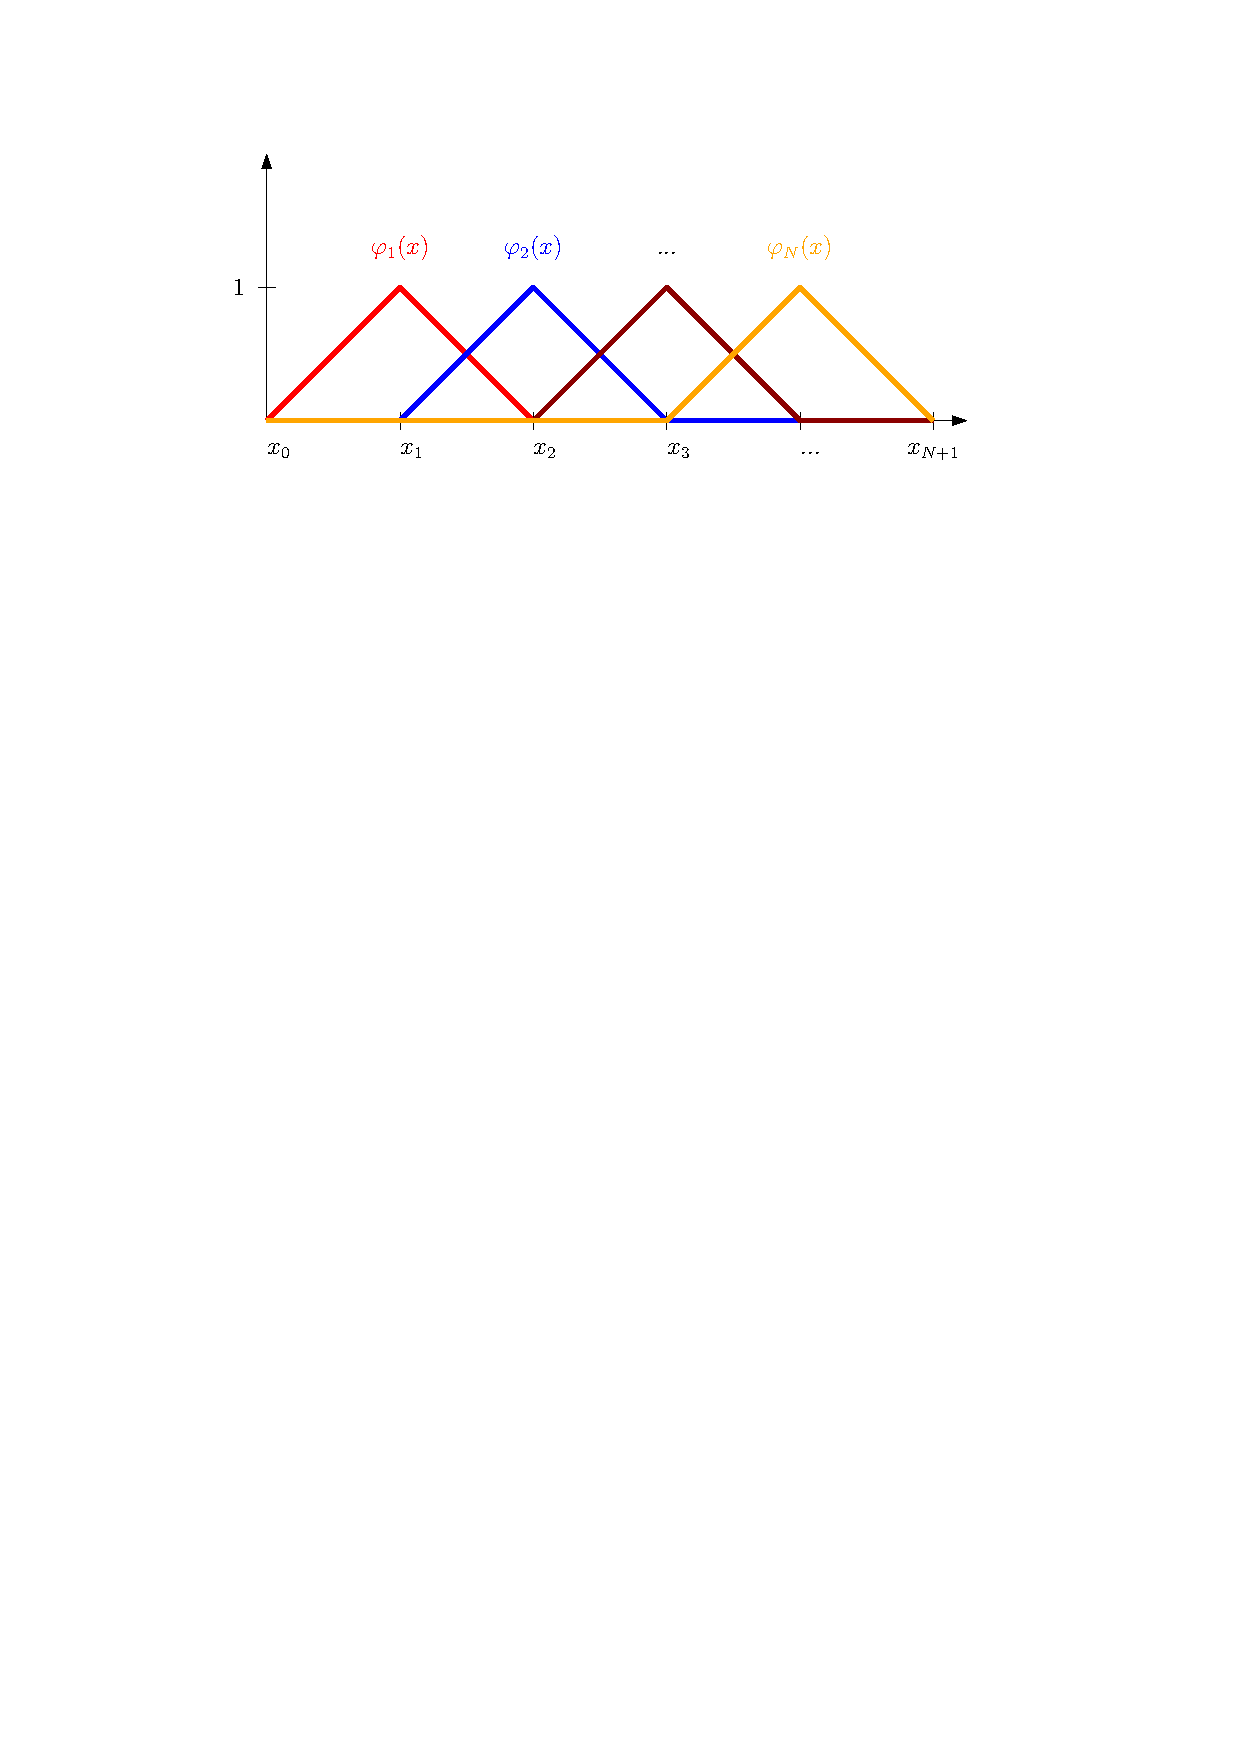
\includegraphics{base_1d_lin}
\caption{Bázové funkce pro prostor po částech lineárních funkcí.}
\label{fig:base_1d_lin}
\end{figure}
Prvky matice $\tn A\in\R^{N\times N}$ a vektoru $\vc b\in\R^{N}$ mají tvar
\[ a_{ij}=\int_0^1\varphi_j'(x)\varphi_i(x), \]
\[ b_i = \int_0^1 f(x)\varphi_i(x)\d x. \]
Je zřejmé, že $a_{ij}$ je nulové, pokud se indexy $i$ a $j$ liší více než o 1, neboť v takovém případě je v každém bodě intervalu $(0,1)$ alespoň jedna z funkcí $\varphi_i$, $\varphi_j$ nulová. Matice $\tn A$ proto bude třídiagonální, a tedy řídká.
Platí:
\begin{align*}
a_{jj} &= \int_{x_{j-1}}^{x_j}\varphi_j'(x)^2\d x + \int_{x_j}^{x_{j+1}}\varphi_j'(x)^2\d x
= \int_{x_{j-1}}^{x_j}\frac1{h_{j-1}^2}\d x + \int_{x_j}^{x_{j+1}}\frac1{h_j^2}\d x\\
&= \frac1{h_{j-1}} + \frac1{h_j},~j=1,...,N,\\\\
a_{j,j-1} &= a_{j-1,j} = \int_{x_{j-1}}^{x_j}\varphi_{j-1}'(x)\varphi_j'(x)\d x\\
&= \int_{x_{j-1}}^{x_j}\frac{(-1)}{h_{j-1}^2} \d x = -\frac1{h_{j-1}}, j=2,...,N.
\end{align*}
V případě ekvidistantního dělení ($h=h_j$ $\forall j=1,...,N$) máme
\[ \tn A = \frac{1}{h}\begin{pmatrix}2 & -1 & \\-1 & 2 & -1\\\ddots&\ddots&\ddots\\&-1 & 2 & -1\\&& -1 & 2\end{pmatrix}. \]
Protože bilineární forma $(a,u,v)$ je symetrická a eliptická, je také $\tn A$ symetrická a pozitivně definitní.
Soustava $\tn A\vc\xi=\vc b$ má řešení pro každý vektor $\vc b$ a řešením Galerkinovy úlohy je funkce $u_h(x):=\sum_{i=1}^N\xi_i\varphi_i(x)$.
Hodnoty $\xi_i$ jsou zároveň hodnotami funkce $u_h$ v bodech $x_i$.

Podobně jako ve Větě \ref{th:cea} lze ukázat, že platí odhad chyby
\begin{equation}\label{eq:error_est_laplace_dir}
\forall v_h\in V_h:~\norm{u'-u_h'}_2 \le \norm{u'-v_h'}_2,
\end{equation}
takže $u_h$ je zároveň nejlepší aproximace slabého řešení $u$ v prostoru po částech lineárních funkcí.
Zvolme nyní vhodnou funkci $v_h$, abychom odhad chyby \eqref{eq:error_est_laplace_dir} vyjádřili kvantitativně.
Položíme $v_h:=\tilde u_h$, kde $\tilde u_h$ je interpolanta $u$ (po částech lineární funkce taková, že $\tilde u_h(x_i)=u(x_i)$, $i=0,...,N+1$).
Pak z teorie Lagrangeovy interpolace víme, že platí
\[ |u'(x)-\tilde u_h'(x)|\le h\max_{y\in[0,1]}|u''(y)| ~\forall x\in[0,1]. \]
Je-li funkce $u$ třídy $C^2([0,1])$, pak dostáváme odhad
\[ \norm{u'-u_h'}_2 \le \norm{u'-\tilde u_h'}_2 \le h\max_{y\in[0,1]}|u''(y)|, \]
který říká, že chyba Galerkinovy aproximace měřená jako $L^2$ norma rozdílu derivací je řádu $O(h)$.


\subsection{Lineární prvky ve vyšší dimenzi}

Pro oblasti v $\R^2$ a $\R^3$ se Galerkinova metoda liší v konstrukci podprostoru $V_h$.
Předpokládejme, že oblast $\Omega$ je polygonální, resp. polyhedrální.
Rozdělme $\Omega$ na nepřekrývající se trojúhelníky, resp. čtyřstěny (tzv. elementy).
Označme $h$ jako průměr největšího elementu.
Množinu všech elementů (triangulace oblasti $\Omega$) budeme značit $\mathcal T_h$.

Je-li slabá formulace zavedena v prostoru $V=H^1_0(\Omega)$, pak prostor $V_h$ můžeme definovat jako množinu
\[ V_h:=\{v_h\in C(\overline\Omega);~\forall K\in\mathcal T_h:~ v_h\mbox{ je lineární na }K,~v_h=0\mbox{ na }\partial\Omega\} \]
všech spojitých po částech lineárních funkcí na $\overline\Omega$.
Na jednom trojúhelníku, resp. čtyřstěnu, je lineární funkce jednoznačně určena svými hodnotami ve vrcholech.
Hodnoty ve všech vrcholech $\{\vc x_i\}_{i=1}^N$ pak tvoří stupně volnosti.
Bázové funkce $\{\varphi_i\}_{i=1}^N$ volíme tak, aby $\varphi_i(\vc x_j)=\delta_{ij}$ (viz Obr. \ref{fig:base_2d_lin}).
\begin{figure}[h]
\centering
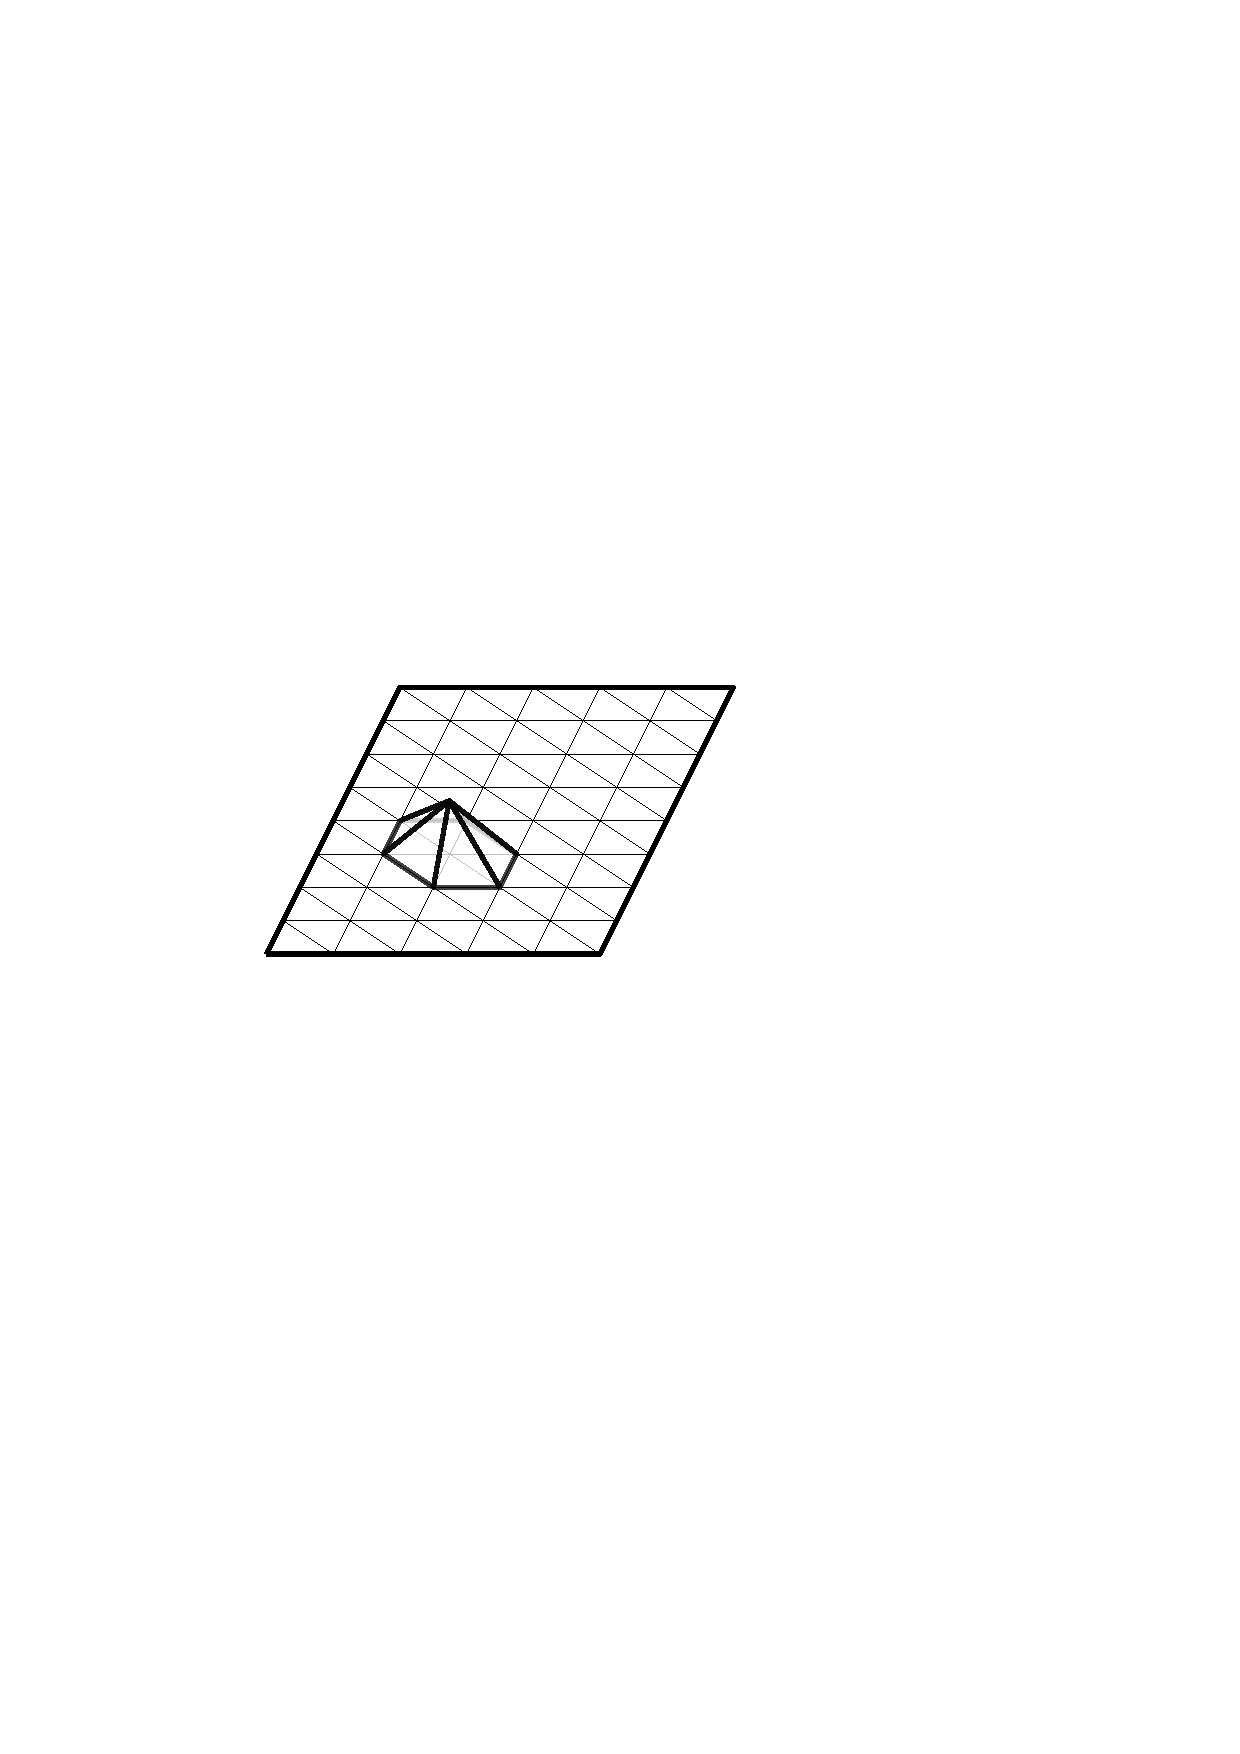
\includegraphics{base_2d_lin}
\caption{Příklad bázové funkce pro prostor po částech lineárních funkcí na 2D oblasti.}
\label{fig:base_2d_lin}
\end{figure}


% \section{Značení}
% 
% Níže jsou uvedeny a vysvětleny v textu často používané symboly.
% 
% \begin{tabular}{ll}
% \bf symbol & \bf význam\\
% \hline
% $\N$ & množina přirozených čísel (1, 2, 3, \ldots)\\
% $\Z$ & množina celých čísel\\
% $\Q$ & množina racionálních čísel\\
% $\R$ & množina reálných čísel\\
% $\C$ & množina komplexních čísel\\
% $A\subset B$ & $A$ je částí (podmnožinou) $B$\\
% $A\cap B$ & průnik\\
% $A\cup B$ & sjednocení\\
% $A\setminus B$ & rozdíl množin\\
% $A\times B$ & kartézský součin\\
% $(a_1,\ldots,a_n)$ & uspořádaná $n$-tice\\
% $(a,b)$ & otevřený interval\\
% $[a,b]$ & uzavřený interval
% \end{tabular}





